\documentclass[table]{beamer}


% Customize slide appearance
\mode<presentation>
{
  \usetheme{Warsaw}
  \setbeamercovered{transparent}
}

\usepackage[english]{babel}
\usepackage{times}
\usefonttheme[onlymath]{serif} 
\setbeamertemplate{navigation symbols}{}

% You can add any graphics to every slide by following command:
% \logo{\resizebox{0.1\textwidth}{!}{\includegraphics{col_small}}}
% \logo{\resizebox{0.2\textwidth}{!}{\includegraphics{imperialblue}}}

% Uncomment this, if you want the table of contents before each subsection.
% However, to edit slides in TeXWord avoiding this feature is good idea.
% \AtBeginSubsection[]
% {
%   \begin{frame}<beamer>
%     \frametitle{Outline}
%     \tableofcontents[currentsection,currentsubsection]
%   \end{frame}
% }

% If you wish to uncover everything in a step-wise fashion, uncomment
% the following command: 
%\beamerdefaultoverlayspecification{<+->}
\xdefinecolor{keyword}{rgb}{0,0,1}
\xdefinecolor{ctext}{rgb}{0.64,0.08,0.08}
\xdefinecolor{cline}{rgb}{0.17,0.57,0.69}
\xdefinecolor{comment}{rgb}{0,0.5,0.0}
\newif\ifschigh\schighfalse
\newcommand{\kw}[1]{\ifschigh\textcolor{red}{#1}\else\textcolor{keyword}{#1}\fi}
\newcommand{\kt}[1]{\ifschigh\textcolor{red}{#1}\else\textcolor{ctext}{#1}\fi}
\newcommand{\kc}[1]{\ifschigh\textcolor{red}{#1}\else\textcolor{comment}{#1}\fi}
\addtobeamertemplate{alerted text begin}{\global\schightrue%
}{}
\defbeamertemplate*{alerted text end}{default}{\global\schighfalse%
}

\newcounter{sckll}
\newcommand{\kr}{\setcounter{sckll}{1}}
\newcommand{\krr}[1]{\setcounter{sckll}{#1}}
\newcommand{\klvalue}{\ifnum\value{sckll}<10{\hphantom{0}}\fi\arabic{sckll}\addtocounter{sckll}{1}}
%\newcommand{\kl}{\ifschigh\textcolor{red}{\klvalue}\else\textcolor{cline}{\klvalue}\fi\hspace{2ex}}
\newcommand{\kl}{}

\newcounter{scpl}
\newcommand{\kp}{\arabic{scpl}\addtocounter{scpl}{2}}
\newcommand{\kpr}{\setcounter{scpl}{3}}

\let\oldurl=\url
\renewcommand{\url}[1]{\textcolor{blue}{\oldurl{#1}}}

\usepackage{tikz, pgfbaseplot, pgflibrarysnakes,pgflibraryarrows}

\begin{document}

% Title Data. We keep it after \begin{document} 
% to enable editing text in BaKoMa TeX Word.

\title[C for Science - Lecture 4]{Computing in C for Science}
\subtitle{Lecture 4 of 5}

% Use the \inst command to identify several affiliations.
\author[Steven Capper]{Dr. Steven Capper \\ {\tt steven.capper99@imperial.ac.uk}\\
\url{http://www2.imperial.ac.uk/~sdc99/ccourse/}}

\date{$7^\text{th}$ December 2011 }

\subject{C for Science} % Should be passed to PDF [YNI]
{
\logo{\includegraphics[width=0.30\textwidth]{imperialblue}}
\begin{frame}
  \titlepage
\end{frame}
}

\begin{frame}[fragile]
\frametitle{Cryptic C}
There are shortcuts in the C language that allow for concise code.
\begin{enumerate}
\item Incrementing by 1. Pre-increment, and post-increment.\\
\begin{tabular}{l l}
\tt ++i& Increment {\tt i} by 1, then use it.\\
\tt i++& Use {\tt i}, then increment it by 1.
\end{tabular}
\item Increment by another variable.\\
\begin{tabular}{r l}
Normal code:&\tt sum = sum + v[i];\\
Terse code:&\tt sum += v[i];
\end{tabular}
\end{enumerate}
An example:\\
\begin{semiverbatim}
   \kw{for} (i=0; i < N; i++)
      sum += v[i];
\end{semiverbatim}
\end{frame}

\begin{frame}
\frametitle{More Shorthand}
\begin{tabular}{l l}
\tt --i;&decrement {\tt i} by 1.\\
\tt sum -= v[i];&means {\tt sum = sum - v[i];}\\
\tt sum *= v[i];&means {\tt sum = sum * v[i];}\\
\tt sum /= v[i];&means {\tt sum = sum / v[i];}\\
\tt sum \%= 2;&means {\tt sum = sum \% 2;}
\end{tabular}
Other operators can also be abbreviated this way.
\begin{exampleblock}{Inline {\tt if}}
The following code:
\begin{center}
\tt \kw{if} (r1 > r2) maxr = r1; \kw{else} maxr = r2;
\end{center}
can be abbreviated:
\begin{center}
\tt maxr = (r1 > r2) ? r1 : r2;
\end{center}
\end{exampleblock}
\end{frame}

\begin{frame}
\frametitle{Matrices - Details}
\framesubtitle{For matrices allocated in the previous lecture}
\begin{tabular}{l l}
\tt matrix & points to a matrix\\
\tt matrix[0]& points to the first row of the matrix\\
\tt matrix[0][0]&The top left element of the matrix
\end{tabular}\\
\vspace{0.2in}
Which have the following types:\\
\begin{tabular}{l l}
\tt matrix& \tt \kw{double} **\\
\tt matrix[0]&\tt \kw{double} *\\
\tt matrix[0][0]& \tt \kw{double}
\end{tabular}
\end{frame}

\begin{frame}[fragile]
\frametitle{Higher Dimensional Arrays}
\begin{semiverbatim}
\tiny
\kr\kl\kw{double} *** alloc3Tensor(\kw{unsigned int} dim)
\kl\{
\kl   \kw{unsigned int} i, j;
\kl   \kw{double} *** tensor;
\kl   tensor = (\kw{double} ***) malloc(dim*\kw{sizeof}(\kw{double} **));
\kl   \kw{if} (!tensor) \kw{return} NULL;
\kl   tensor[0] = (\kw{double} **) malloc(dim*dim*\kw{sizeof}(\kw{double} *));
\kl   \kw{if} (!tensor[0])
\kl   \{
\kl      free(tensor);
\kl      \kw{return} NULL;
\kl   \}
\kl   tensor[0][0] = (\kw{double} *) malloc(dim*dim*dim*\kw{sizeof}(\kw{double}));
\kl   \kw{if} (!tensor[0][0])
\kl   \{
\kl      free(tensor[0]); free(tensor);
\kl      \kw{return} NULL;
\kl   \}
\kl   \kw{for} (i = 1; i < dim; i++)
\kl      tensor[0][i] = tensor[0][i-1]+dim;
\kl   \kw{for} (i = 1; i < dim; i++)
\kl   \{
\kl      tensor[i] = tensor[i-1] + dim;
\kl      tensor[i][0] = tensor[i-1][0] + dim * dim;
\kl      \kw{for} (j = 1; j < dim; j++)
\kl         tensor[i][j] = tensor[i][j-1] + dim;
\kl   \}
\kl   \kw{return} tensor;
\kl\}
\end{semiverbatim}
\end{frame}

\begin{frame}[fragile]
\frametitle{More Multi-Index}
\begin{itemize}
\item The 3D array behaves as expected:\\
\begin{center}
\tt tensor[i][j][k] = 0.5;
\end{center}
\item The array can be freed with:
\begin{semiverbatim}
\kw{void} free3Tensor(\kw{double} *** tensor)
\{
   free(tensor[0][0]);
   free(tensor[0]);
   free(tensor);
\}
\end{semiverbatim}
\end{itemize}
\end{frame}

\begin{frame}
\frametitle{More Elaborate Data Structures}
\begin{itemize}
\item In C we are able to manipulate data directly, this has allowed us to partition a contiguous array of memory into matrix rows.
\item We needn't restrict ourselves to structures where the number of elements per row is constant, one example is Pascal's triangle:\\
\begin{center}
\tt1\\\tt1  2  1\\\tt1  3  3  1\\\tt1  4  6  4  1\\$\vdots$
\end{center}
\end{itemize}
\end{frame}

\begin{frame}[fragile]
\begin{semiverbatim}
\scriptsize
\kr\kl\kw{int} main()
\kl\{
\kl   \kw{unsigned int} size = 10, r, c;
\kl   \kw{int} ** pasc;
\kl   pasc = (\kw{int} **) malloc(size*sizeof(int));
\kl   pasc[0] = (\kw{int} *) malloc(size*(size+1)*sizeof(int)/2);
\kl   \kc{/* check the mallocs */}
\kl   \kw{for} (r=1; r < size; r++) pasc[r] = pasc[r-1]+r;
\kl   pasc[0][0] = 1;
\kl   \kw{for} (r = 1; r < size; r++)
\kl   \{
\kl      \kw{for} (c = 1; c < r; c++)
\kl         pasc[r][c] = pasc[r-1][c-1]+pasc[r-1][c];
\kl      pasc[r][0] = 1; pasc[r][r] = 1;
\kl   \}
\kl   \kw{for} (r=0; r < size; r++)
\kl   \{
\kl      \kw{for} (c = 0; c < r+1; c++)
\kl         printf(\kt{"\%3d "}, pasc[r][c]);
\kl      printf(\kt{"\\n"});
\kl   \}
\kl   free(pasc[0]);
\kl   free(pasc);
\kl   \kw{return} 0;
\kl\}
\end{semiverbatim}
\end{frame}

\begin{frame}[fragile]
\frametitle{Pascal's Triangle}
\begin{itemize}
\item The program outputs:
\vspace{-0.2in}
\begin{semiverbatim}
\small
  1
  1   1
  1   2   1
  1   3   3   1
  1   4   6   4   1
  1   5  10  10   5   1
  1   6  15  20  15   6   1
  1   7  21  35  35  21   7   1
  1   8  28  56  70  56  28   8   1
  1   9  36  84 126 126  84  36   9   1
\end{semiverbatim}
\item Whilst in memory, the data structure looks like:
\begin{tabular}{|c|c|c|c|c|c|c|c|c|c|c|}
\hline
\tt1&\tt1&\tt1&\tt1&\tt2&\tt1&\tt1&\tt3&\tt3&\tt1&$\cdots$\\
\hline
\end{tabular}
\end{itemize}
\end{frame}

\begin{frame}[fragile]
\frametitle{Custom Data Types}
Recall, when dealing with files we used:
\begin{semiverbatim}
FILE * file;
file = fopen (\kt{"myfile.txt"}, \kt{"r"});
\end{semiverbatim}
{\tt FILE} is in fact a custom data type, with its own size:
\begin{semiverbatim}
\kw{\#include} \kt{<stdio.h>}

\kw{int} main()
\{
   printf(\kt{"sizeof(FILE) = \%d\\n"}, \kw{sizeof}(FILE));
   \kw{return} 0;
\}
\end{semiverbatim}
\end{frame}

\begin{frame}[fragile]
\frametitle{Except from MS - \kt{\tt <stdio.h>}}
(From Visual Studio 2008)
\begin{semiverbatim}
\kw{struct} _iobuf \{
   \kw{char} *_ptr;
   \kw{int}   _cnt;
   \kw{char} *_base;
   \kw{int}   _flag;
   \kw{int}   _file;
   \kw{int}   _charbuf;
   \kw{int}   _bufsiz;
   \kw{char} *_tmpfname;
   \};
\kw{typedef struct} _iobuf FILE;
\end{semiverbatim}
\end{frame}

\begin{frame}[fragile]
\frametitle{{\tt typedef} Structures : Custom Data Types}
\begin{itemize}
\item {\tt FILE} is a custom data type defined in \kt{\tt <stdio.h>}.
\item It is comprised of elements of different, known, types.
\item Each element of the {\tt FILE} \emph{structure} has its own name.
\end{itemize}

Let's consider a structure of our own, one of the simplest examples is a complex number:
\begin{columns}
\begin{column}{5cm}
\begin{semiverbatim}
\kw{typedef struct}
\{
   \kw{double} real;
   \kw{double} imag;
\} complex;
\end{semiverbatim}
\end{column}
\begin{column}{5cm}
\begin{alertblock}{C99}
C99 fully supports its own {\tt complex}
type.
\end{alertblock}
\end{column}
\end{columns}
\end{frame}

\begin{frame}[fragile]
\frametitle{{\tt typedef} Structures - II}
Definitions of structures take the following form:
\begin{semiverbatim}
   \kw{typedef struct}
   \{
      \emph{elementType} \emph{elementName};
      \emph{elementType} \emph{elementName};
      \vdots
   \} \emph{structureTypeName} ;
\end{semiverbatim}
\end{frame}

\begin{frame}
\frametitle{Handling Structures}
\begin{enumerate}
\item A structure may be an argument to a function.
\item A function may return a structure.
\item A pointer may point to a structure.
\item Structures are referenced as normal: {\tt \&name}.
\item Elements of a structure are references as: {\tt \&name.element}.
\item A pointer to a structure may be passed to a function.
\item If {\tt p} is a pointer to a structure, then {\tt p->member} allows us to access it's members.
\end{enumerate}
\end{frame}

\begin{frame}[fragile]
\frametitle{Example Function Applying to Structures}
\vspace{-0.2in}
\begin{semiverbatim}
\scriptsize
\kr\kl\kw{\#include} \kt{<stdio.h>}
\kl
\kl\kw{typedef struct}
\kl\{
\kl   \kw{double} real;
\kl   \kw{double} imag;
\kl\} complex;
\kl
\kl\kw{void} printComplex(complex * mc)
\kl\{
\kl   printf(\kt{"\%lg + \%lgi\\n"}, mc->real, mc->imag);
\kl\}
\kl
\kl\kw{int} main()
\kl\{
\kl   complex c1 = \{1.0, 0.5\}; \kc{/* assignment at declaration */}
\kl   printComplex(&c1);       \kc{/* pass pointer to struct */}
\kl   c1.real = 10.0;          \kc{/* piecewise assignment */}
\kl   printComplex(&c1);
\kl   \kw{return} 0;
\kl\}
\end{semiverbatim}
\end{frame}

\begin{frame}
\frametitle{More Structures}
\begin{itemize}
\item Passing structures via pointer is usually more efficient.
\item Assignment can be done at declaration or after.
\item In C we are not allowed to overload operators, so the following won't work:
\begin{center}
{\tt c1 = c2 + c3;} (where {\tt c1} and {\tt c2} are {\tt complex})
\end{center}
so we need to do something like:
\begin{center}
{\tt complexAdd(\&c1, \&c2, \&c3);}
\end{center}
\item Arrays of {\tt \kw{struct}}s are allowed (so matrices can consist of complex numbers for example).
\item Structures can contain structures as elements.
\end{itemize}
\end{frame}

\begin{frame}
\frametitle{Complex Number Support in C/C++}
\begin{exampleblock}{C++}
Complex numbers are supported in C++ as {\tt \kw{class}}es, also the operators are overloaded properly too meaning any code which uses them will be concise.
(look in {\tt \kt{<complex>}}).
\end{exampleblock}

\begin{block}{C99}
Complex numbers are supported as a native data type (not {\tt \kw{struct}}) in C99. Unfortunately not many compilers support this. GNU C, fully supports complex numbers (see {\tt \kt{<complex.h>}}).
\end{block}

\begin{alertblock}{C90}
Complex number support in C90 is non-existent. I would recommend either third party libraries or a switch to C99/C++ for heavy complex number use.
\end{alertblock}
\end{frame}

\begin{frame}[fragile]
\frametitle{Another Example {\tt \kw{struct}} - from {\tt \kt{<time.h>}}}
\begin{semiverbatim}
\footnotesize
\kw{struct} tm
\{
   \kw{int} tm_sec;     \kc{/* seconds after the minute - [0,59] */}
   \kw{int} tm_min;     \kc{/* minutes after the hour - [0,59] */}
   \kw{int} tm_hour;    \kc{/* hours since midnight - [0,23] */}
   \kw{int} tm_mday;    \kc{/* day of the month - [1,31] */}
   \kw{int} tm_mon;     \kc{/* months since January - [0,11] */}
   \kw{int} tm_year;    \kc{/* years since 1900 */}
   \kw{int} tm_wday;    \kc{/* days since Sunday - [0,6] */}
   \kw{int} tm_yday;    \kc{/* days since January 1 - [0,365] */}
   \kw{int} tm_isdst;   \kc{/* daylight savings time flag */}
\};
\end{semiverbatim}
\end{frame}

\begin{frame}
\frametitle{Compilation}
\begin{itemize}
\item As seen in the first lecture, C programs are \emph{compiled} into a low level (machine specific language).
\item This language is called \emph{assembly language}.
\item On PCs and Macs Intel x86 assembler is ubiquitous.
\item Most C compilers allow you to view the assembler that they generate.
\end{itemize}
\end{frame}

\begin{frame}[fragile]
\frametitle{{\tt addMatrices} revisited - C code}
From the last lecture we saw a function to add two matrices together:
\begin{semiverbatim}
\small
\kw{void} addMatrices(\kw{double} ** matrixA, \kw{double} ** matrixB,
                 \kw{double} ** matrixR,
                 \kw{unsigned int} rows, \kw{unsigned int} cols)
\{
   \kw{unsigned int} i, j;
   \kw{for} (i = 0; i < rows; i++)
      \kw{for} (j = 0; j < cols; j++)
         matrixR[i][j] = matrixA[i][j]+matrixB[i][j];
\}
\end{semiverbatim}
When we compile this, we get...
\end{frame}

\begin{frame}[fragile]
\frametitle{{\tt addMatrices} revisited - when compiled...}
\begin{columns}
\begin{column}{5cm}
\vspace{-0.2in}
\begin{semiverbatim}
\tiny
_addMatrices PROC
; 35   : \{
        push    ebp
        mov     ebp, esp
        sub     esp, 216
        push    ebx
        push    esi
        push    edi
        lea     edi, DWORD PTR [ebp-216]
        mov     ecx, 54
        mov     eax, -858993460
        rep stosd
; 36   :        unsigned int i, j;
; 37   :        for (i = 0; i < rows; i++)
        mov     DWORD PTR _i$[ebp], 0
        jmp     SHORT $LN6@addMatrice
$LN5@addMatrice:
        mov     eax, DWORD PTR _i$[ebp]
        add     eax, 1
        mov     DWORD PTR _i$[ebp], eax
$LN6@addMatrice:
        mov     eax, DWORD PTR _i$[ebp]
        cmp     eax, DWORD PTR _rows$[ebp]
        jae     SHORT $LN4@addMatrice
; for (j = 0; j < rows; j++)
        mov     DWORD PTR _j$[ebp], 0
        jmp     SHORT $LN3@addMatrice
$LN2@addMatrice:
        mov     eax, DWORD PTR _j$[ebp]
        add     eax, 1
        mov     DWORD PTR _j$[ebp], eax
\end{semiverbatim}
\end{column}
\begin{column}{5cm}
\vspace{-0.2in}
\begin{semiverbatim}
\tiny
$LN3@addMatrice:
        mov     eax, DWORD PTR _j$[ebp]
        cmp     eax, DWORD PTR _rows$[ebp]
        jae     SHORT $LN1@addMatrice
;matrixR[i][j] = matrixA[i][j]+matrixB[i][j];
        mov     eax, DWORD PTR _i$[ebp]
        mov     ecx, DWORD PTR _matrixA$[ebp]
        mov     edx, DWORD PTR [ecx+eax*4]
        mov     eax, DWORD PTR _i$[ebp]
        mov     ecx, DWORD PTR _matrixB$[ebp]
        mov     eax, DWORD PTR [ecx+eax*4]
        mov     ecx, DWORD PTR _j$[ebp]
        mov     esi, DWORD PTR _j$[ebp]
\textcolor{red}{        fld     QWORD PTR [edx+ecx*8]}
\textcolor{red}{        fadd    QWORD PTR [eax+esi*8]}
        mov     edx, DWORD PTR _i$[ebp]
        mov     eax, DWORD PTR _matrixR$[ebp]
        mov     ecx, DWORD PTR [eax+edx*4]
        mov     edx, DWORD PTR _j$[ebp]
\textcolor{red}{        fstp    QWORD PTR [ecx+edx*8]}
        jmp     SHORT $LN2@addMatrice
$LN1@addMatrice:
        jmp     SHORT $LN5@addMatrice
$LN4@addMatrice:
        pop     edi
        pop     esi
        pop     ebx
        mov     esp, ebp
        pop     ebp
        ret     0
_addMatrices ENDP
\end{semiverbatim}
\end{column}
\end{columns}
\end{frame}

\begin{frame}
\frametitle{Optimisation}
\begin{itemize}
\item A few lines of C becomes $>30$ lines of assembler (only three of which are actually floating point instructions!).
\item It is possible to write a much smaller assembler routine by hand $\approx$10-20 instructions long.
\item This would run $\approx$3 times quicker than the C compiled routine (this is a general rule of thumb).
\item Any custom assembly code would only target a very specific chip, however.
\end{itemize}
\end{frame}

\begin{frame}
\frametitle{Optimisation II}
\begin{itemize}
\item Rather than rewrite the assembly code, it is easier to ask the C compiler to perform code optimisation itself.
\item By default C will compile the code as it appears (the exact order of operations is preserved etc), this is aids debugging.
\item C compilers can be told to optimise their code in the following ways:
\begin{center}
\begin{tabular}{l p{220pt}}
MSVC&Project configuration options can be set, defaults in ``Release'' build do a good job.\\
gcc&The {\tt -O} command line flags influence optimisation, {\tt -O0} means ``off'' whilst {\tt -O3} means ``extremely aggressive''.
\end{tabular}
\end{center}
\end{itemize}
\end{frame}

\begin{frame}[fragile]
\frametitle{Optimisation Example - Visual Studio 2008}
\begin{columns}
\begin{column}{5cm}
\begin{center}
Debug Build
\end{center}
\begin{semiverbatim}
\tiny
$LN2@addMatrice:
        mov     eax, DWORD PTR _j$[ebp]
        add     eax, 1
        mov     DWORD PTR _j$[ebp], eax
$LN3@addMatrice:
        mov     eax, DWORD PTR _j$[ebp]
        cmp     eax, DWORD PTR _rows$[ebp]
        jae     SHORT $LN1@addMatrice
;matrixR[i][j] = matrixA[i][j]+matrixB[i][j];
        mov     eax, DWORD PTR _i$[ebp]
        mov     ecx, DWORD PTR _matrixA$[ebp]
        mov     edx, DWORD PTR [ecx+eax*4]
        mov     eax, DWORD PTR _i$[ebp]
        mov     ecx, DWORD PTR _matrixB$[ebp]
        mov     eax, DWORD PTR [ecx+eax*4]
        mov     ecx, DWORD PTR _j$[ebp]
        mov     esi, DWORD PTR _j$[ebp]
\textcolor{red}{        fld     QWORD PTR [edx+ecx*8]}
\textcolor{red}{        fadd    QWORD PTR [eax+esi*8]}
        mov     edx, DWORD PTR _i$[ebp]
        mov     eax, DWORD PTR _matrixR$[ebp]
        mov     ecx, DWORD PTR [eax+edx*4]
        mov     edx, DWORD PTR _j$[ebp]
\textcolor{red}{        fstp    QWORD PTR [ecx+edx*8]}
        jmp     SHORT $LN2@addMatrice
\end{semiverbatim}
\end{column}
\begin{column}{5cm}
\begin{center}
Release Build
\end{center}
\begin{semiverbatim}
\tiny
;matrixR[i][j] = matrixA[i][j]+matrixB[i][j];
\textcolor{red}{                fld     QWORD PTR [edx+eax]}
\textcolor{red}{                fadd    QWORD PTR [eax]}
\textcolor{red}{                fstp    QWORD PTR [esi+eax]}
        add     eax, 8
        dec     ebx
        jne     SHORT $LL3@addMatrice
\end{semiverbatim}
\vspace{1.55in}
\end{column}
\end{columns}
\end{frame}

\begin{frame}
\frametitle{Bits and Bytes}
\begin{columns}
\begin{column}{5cm}
\begin{block}{Bytes}
Smallest \emph{addressable} unit of memory, each byte is composed of eight bits.
\end{block}
\end{column}
\begin{column}{5cm}
\begin{block}{Bits}
These are the smallest units of computer memory, each bit can be either 0 or 1.
\end{block}
\end{column}
\end{columns}
\vspace{0.2in}
\begin{itemize}
\item Addressing bits individually requires some extra operations to be carried out.
\item There are good reasons for accessing data at the bit-level however.
\end{itemize}
\end{frame}

\begin{frame}
\frametitle{Efficient Data Packing}
\begin{block}{Given a 32 million base pair chromosome}
\begin{tabular}{l l}
It will require: &$\approx$64 megabytes to store as {\tt short}\\
&$\approx$32 megabytes to store as {\tt char} (next lecture)\\
&$\approx$8 megabytes to store as bit data.
\end{tabular}
(i.e. a 2-4 year research lead if following Moore's Law).
\end{block}
\begin{block}{Computer Graphics}
Given a monochrome print image of 2400 dpi rendered over 80 square inches gives $\approx 500,000,000$ dots. This takes up:
\begin{center}
\begin{tabular}{l}
$\approx$1 gigabyte if using {\tt short}\\
$\approx$64 megabytes if using bits.
\end{tabular}
\end{center}
\end{block}
\end{frame}

\begin{frame}
\frametitle{Bit Manipulation Friendly Data Types}
As seen before the unsigned integer data types have values ranging from 0 to $2^n-1$ where $n$ is the number of bits in the data type. Some examples (for my machine):
\begin{center}
\rowcolors[]{1}{blue!20}{blue!10}
\begin{tabular}{l c}
\bf Data Type&\bf$n$\\
\tt unsigned short& 16\\
\tt unsigned int&32\\
\tt unsigned long int&64\\
\tt unsigned long long int&128
\end{tabular}
\end{center}
Unsigned data types are also desirable for accessing array indices as they can never be negative.
\end{frame}

\begin{frame}
\frametitle{How to Get Them In and Out of The Computer}
\begin{itemize}
\item They can be read using {\tt scanf} and {\tt \kt{"\%u"}}, {\tt \kt{"\%lu"}}
 or {\tt \kt{"\%Lu"}}.
\item They can be printed using {\tt printf} and {\tt \kt{"\%u"}} or {\tt \kt{"\%Lu"}}.
\item We can output to octal (base 8 numbers) using {\tt printf} and {\tt \kt{"\%o"}}
\item Also we can output to hexadecimal (base 16, 0-9 and a-f) using {\tt printf} and {\tt \kt{"\%x"}} or {\tt \kt{"\%X"}}.
\end{itemize}
\begin{block}{Example - byte ({\tt char})}
\begin{tabular}{l l}
Binary&\tt10101011\\
Hexadecimal&\tt AB\\
Decimal&\tt171\\
Octal&\tt253
\end{tabular}
\end{block}
\end{frame}

\begin{frame}
\frametitle{Manipulating Bits within an Unsigned Integer}
\begin{itemize}
\item C can shift all the bits comprising a number a fixed number of places to the left or right.
\item Zeros are propagated in to the vacated spaces.
\item Bits that shift outside, disappear. (i.e. the shift is not cyclic).
\item Bit shifting is accomplished with the {\tt >>} (right) and {\tt <<} (left) operators.
\end{itemize}
For example:
\begin{center}
\tt 1 << 2 = 4\\
\tt 8 >> 3 = 1
\end{center}
\begin{block}{}
Bit shifts are much cheaper than multiplying or dividing by powers of two.
\end{block}
\end{frame}

\begin{frame}
\frametitle{4 Bitwise operators {\tt \&}, {\tt|}, {\tt$\wedge$} and {\tt$\sim$}}
Assuming 0 is false and 1 is true, we have the following bitwise logical operators.
\begin{columns}
\begin{column}{5cm}
\begin{block}{And Operator(\&)}
\begin{tabular}{r|c c c c}
N1&0&0&1&1\\
N2&0&1&0&1\\
\hline
N1 \& N2&0&0&0&1
\end{tabular}
\end{block}

\begin{block}{Exclusive Or({\tt$\wedge$})}
\begin{tabular}{r|c c c c}
N1&0&0&1&1\\
N2&0&1&0&1\\
\hline
N1 {\tt$\wedge$} N2&0&1&1&0
\end{tabular}
\end{block}

\end{column}
\begin{column}{5cm}
\begin{block}{Or Operator({\tt|})}
\begin{tabular}{r|c c c c}
N1&0&0&1&1\\
N2&0&1&0&1\\
\hline
N1 {\tt|} N2&0&1&1&1
\end{tabular}
\end{block}

\begin{block}{Not Operator({\tt$\sim$})}
\begin{tabular}{r|c c}
N1&0&1\\
\hline
{\tt$\sim$}N1&1&0
\end{tabular}
\end{block}
\vspace{0.13in}
\end{column}
\end{columns}
\end{frame}

\begin{frame}
\frametitle{Case Study: The Sieve of Eratosthenes}
\begin{center}
\kpr
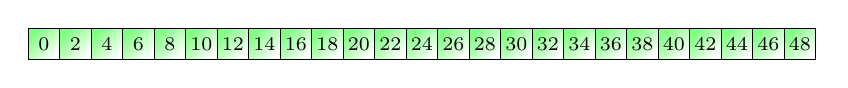
\begin{tikzpicture}[]
\foreach \x in {0.0, 0.4, ..., 9.6}
   \shadedraw [top color=green!50,shading angle=45] (\x,0) rectangle +(0.4,0.4);
\foreach \x in {0.2, 0.6, ..., 10.2}
   \node at (\x, 0.2) {{\scriptsize\kp}};  
\end{tikzpicture}
\end{center}

\begin{center}
\kpr
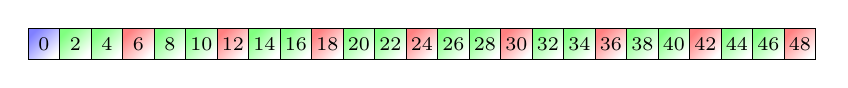
\begin{tikzpicture}[]
\foreach \x in {0.0, 0.4, ..., 9.6}
   \shadedraw [top color=green!50,shading angle=45] (\x,0) rectangle +(0.4,0.4); \shadedraw [top color=blue!50, shading angle=45] (0, 0) rectangle +(0.4,0.4);
\foreach \x in {1.2, 2.4, ..., 9.6}
   \shadedraw [top color=red!50,shading angle=45] (\x,0) rectangle +(0.4,0.4); \foreach \x in {0.2, 0.6, ..., 10.2}
   \node at (\x, 0.2) {{\scriptsize\kp}};  
\end{tikzpicture}
\end{center}

\begin{center}
\kpr
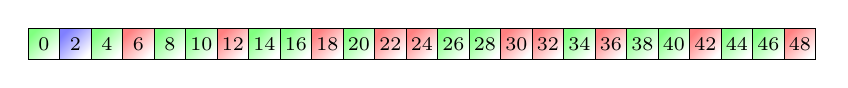
\begin{tikzpicture}[]
\foreach \x in {0.0, 0.4, ..., 9.6}
   \shadedraw [top color=green!50,shading angle=45] (\x,0) rectangle +(0.4,0.4); \shadedraw [top color=blue!50, shading angle=45] (0.4,0) rectangle +(0.4,0.4);
\foreach \x in {1.2, 2.4, ..., 9.6}
   \shadedraw [top color=red!50,shading angle=45] (\x,0) rectangle +(0.4,0.4);
\foreach \x in {2.4, 4.4, ..., 9.6}
   \shadedraw [top color=red!50,shading angle=45] (\x,0) rectangle +(0.4,0.4);
\foreach \x in {0.2, 0.6, ..., 10.2}
   \node at (\x, 0.2) {{\scriptsize\kp}};  
\end{tikzpicture}
\end{center}

\begin{center}
\kpr
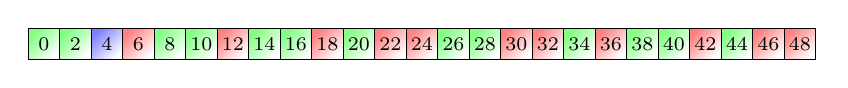
\begin{tikzpicture}[]
\foreach \x in {0.0, 0.4, ..., 9.6}
   \shadedraw [top color=green!50,shading angle=45] (\x,0) rectangle +(0.4,0.4); \shadedraw [top color=blue!50, shading angle=45] (0.8,0) rectangle +(0.4,0.4);
\foreach \x in {1.2, 2.4, ..., 9.6}
   \shadedraw [top color=red!50,shading angle=45] (\x,0) rectangle +(0.4,0.4);
\foreach \x in {2.4, 4.4, ..., 9.6}
   \shadedraw [top color=red!50,shading angle=45] (\x,0) rectangle +(0.4,0.4);
\foreach \x in {3.6, 6.4, ..., 9.6}
   \shadedraw [top color=red!50,shading angle=45] (\x,0) rectangle +(0.4,0.4); \foreach \x in {0.2, 0.6, ..., 10.2}
   \node at (\x, 0.2) {{\scriptsize\kp}};  
\end{tikzpicture}
\end{center}

\begin{center}
\kpr
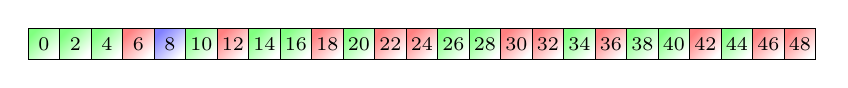
\begin{tikzpicture}[]
\foreach \x in {0.0, 0.4, ..., 9.6}
   \shadedraw [top color=green!50,shading angle=45] (\x,0) rectangle +(0.4,0.4); \shadedraw [top color=blue!50, shading angle=45] (1.6,0) rectangle +(0.4,0.4);
\foreach \x in {1.2, 2.4, ..., 9.6}
   \shadedraw [top color=red!50,shading angle=45] (\x,0) rectangle +(0.4,0.4);
\foreach \x in {2.4, 4.4, ..., 9.6}
   \shadedraw [top color=red!50,shading angle=45] (\x,0) rectangle +(0.4,0.4);
\foreach \x in {3.6, 6.4, ..., 9.6}
   \shadedraw [top color=red!50,shading angle=45] (\x,0) rectangle +(0.4,0.4); \foreach \x in {0.2, 0.6, ..., 10.2}
   \node at (\x, 0.2) {{\scriptsize\kp}};  
\end{tikzpicture}
\end{center}

\begin{center}
\kpr
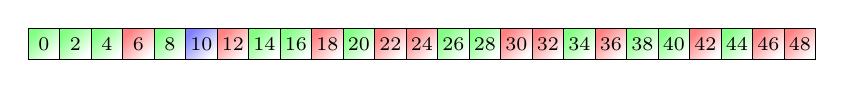
\begin{tikzpicture}[]
\foreach \x in {0.0, 0.4, ..., 9.6}
   \shadedraw [top color=green!50,shading angle=45] (\x,0) rectangle +(0.4,0.4); \shadedraw [top color=blue!50, shading angle=45] (2.0,0) rectangle +(0.4,0.4);
\foreach \x in {1.2, 2.4, ..., 9.6}
   \shadedraw [top color=red!50,shading angle=45] (\x,0) rectangle +(0.4,0.4);
\foreach \x in {2.4, 4.4, ..., 9.6}
   \shadedraw [top color=red!50,shading angle=45] (\x,0) rectangle +(0.4,0.4);
\foreach \x in {3.6, 6.4, ..., 9.6}
   \shadedraw [top color=red!50,shading angle=45] (\x,0) rectangle +(0.4,0.4); \foreach \x in {0.2, 0.6, ..., 10.2}
   \node at (\x, 0.2) {{\scriptsize\kp}};  
\end{tikzpicture}
\end{center}

\begin{center}
\kpr
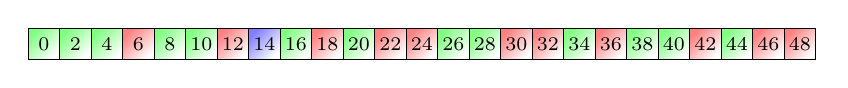
\begin{tikzpicture}[]
\foreach \x in {0.0, 0.4, ..., 9.6}
   \shadedraw [top color=green!50,shading angle=45] (\x,0) rectangle +(0.4,0.4); \shadedraw [top color=blue!50, shading angle=45] (2.8,0) rectangle +(0.4,0.4);
\foreach \x in {1.2, 2.4, ..., 9.6}
   \shadedraw [top color=red!50,shading angle=45] (\x,0) rectangle +(0.4,0.4);
\foreach \x in {2.4, 4.4, ..., 9.6}
   \shadedraw [top color=red!50,shading angle=45] (\x,0) rectangle +(0.4,0.4);
\foreach \x in {3.6, 6.4, ..., 9.6}
   \shadedraw [top color=red!50,shading angle=45] (\x,0) rectangle +(0.4,0.4); \foreach \x in {0.2, 0.6, ..., 10.2}
   \node at (\x, 0.2) {{\scriptsize\kp}};  
\end{tikzpicture}
\end{center}

This gives the primes (we add 2 to the beginning of the list):
\resizebox{\textwidth}{!}{
\begin{tabular}{ccccccccccccccc}
2&3&5&7&11&13&17&19&23&29&31&37&41&43&47
\end{tabular}}
\end{frame}

\begin{frame}
\frametitle{The Sieve of Eratosthenes: In C}
\begin{itemize}
\item When implementing this in C it makes sense to use a bit to indicate `primeness' of a number.
\item The smallest addressable unit of memory in C is the {\tt \kw{char}} which consists of 8 bits.
\item We therefore need to perform \emph{masking} to isolate individual bits.
\end{itemize}
\begin{block}{Masking}
We access the $j^\mathrm{th}$ bit of a variable {\tt x} as follows:
\begin{center}
\begin{tabular}{l l}
\tt \kw{if}(x \& (1 << j))&Check to see if it's set\\
\tt x |= (1 << j)& To set the bit\\
\tt x \&= $\sim$(1 << j)&To clear the bit
\end{tabular}
\end{center}
\end{block}
\end{frame}

\begin{frame}[fragile]
\frametitle{The Sieve of Eratosthenes: Implementation}
\vspace{-0.2in}
\begin{semiverbatim}
\scriptsize
\kr\kl\kw{void} findPrimes(NUM_TYPE * Prime_List, \kw{int} max_num)
\kl\{
\kl   \kw{int} current_num = 3;
\kl   NUM_TYPE Mask=1;
\kl
\kl   \kw{while}(current_num*current_num <= max_num)
\kl   \{
\kl      \kw{int} Pnum = current_num/(2 * BITS_PER_NUM);
\kl      \kw{int} Pbit = (current_num-Pnum * 2 * BITS_PER_NUM)/2;
\kl      \kc{/* Current Number is prime so strike out multiples */}
\kl      \kw{if}(~Prime_List[Pnum] & (Mask <<Pbit))
\kl      \{
\kl         \kw{int} strike = current_num * current_num;
\kl         \kw{while}(strike <= max_num)
\kl         \{
\kl            \kw{int} Snum = strike/(2*BITS_PER_NUM);
\kl            \kw{int} Sbit = (strike - Snum * 2 * BITS_PER_NUM)/2;
\kl            Prime_List[Snum] |= (Mask << Sbit);
\kl            strike += 2 * current_num;
\kl         \}                       
\kl      \}
\kl      current_num += 2;
\kl   \}
\kl\}
\end{semiverbatim}
\end{frame}

\begin{frame}[fragile]
\frametitle{The Sieve of Eratosthenes : Printing out the Primes}
\begin{semiverbatim}
\small
\kr\kl\kw{void} printPrimes(NUM_TYPE * Prime_List, \kw{int} max_num)
\kl\{
\kl   \kw{int} i;
\kl   NUM_TYPE Mask=1;
\kl
\kl   \kw{for}(i = 3;i <= max_num;i = i+2)
\kl   \{
\kl      \kw{int} Pnum=i/(2*BITS_PER_NUM);
\kl      \kw{int} Pbit=(i-Pnum*2*BITS_PER_NUM)/2;
\kl      \kw{if} (~Prime_List[Pnum] & (Mask <<Pbit))
\kl         printf(\kt{"\%d\\n"}, i);
\kl   \}
\kl\}
\end{semiverbatim}
\end{frame}

\end{document}
